\section{Compiling ForeC for Parallel Execution}
\label{sec:forec_compiling}
The previous section described the language. To be useful, 
the ForeC program must be compiled 
appropriately to exploit the parallelism of the target
hardware architecture. This section describes how the 
ForeC compiler generates code for direct 
execution on a predictable parallel architecture
described in Section~\ref{sec:introduction:pret:multicore}. The
chosen compilation strategy generates code that is 
amenable to static timing analysis and achieves good
execution performance, as benchmarking results in 
Section~\ref{sec:forec_benchmarking} reveal.

\subsection{Overview}
The ForeC compiler can generate code for direct (bare metal) 
execution on the Xilinx MicroBlaze embedded multi-core 
(Section~\ref{sec:introduction:pret:multicore}) 
processor. Later in Section~\ref{sec:forec_compiling:posix}, 
we extend the compiler to generate code for execution 
on an operating system.
Figure~\ref{fig:forec_compiling:overview} is
an overview of the compilation process. The first step 
checks the syntax of the ForeC source code. This includes
checking whether all threads have been defined and whether
all variables accessed by multiple threads have been
declared with the \verb$shared$ qualifier. The second step
translates the ForeC statements into equivalent C code.
Bootup and thread scheduling routines are generated for
each core. The ForeC threads are statically allocated and
statically scheduled on each core.
The final step is to compile the generated 
C program with the GNU C compiler (GNU's 
computed \verb$goto$ extension is used to implement fast
context-switching). This section describes
the generation of C code. 
For brevity, we omit inputs and outputs 
because we follow existing approaches~\cite{timed_compiling_esterel} for
creating the reactive interface.

\begin{figure}
	\centering

	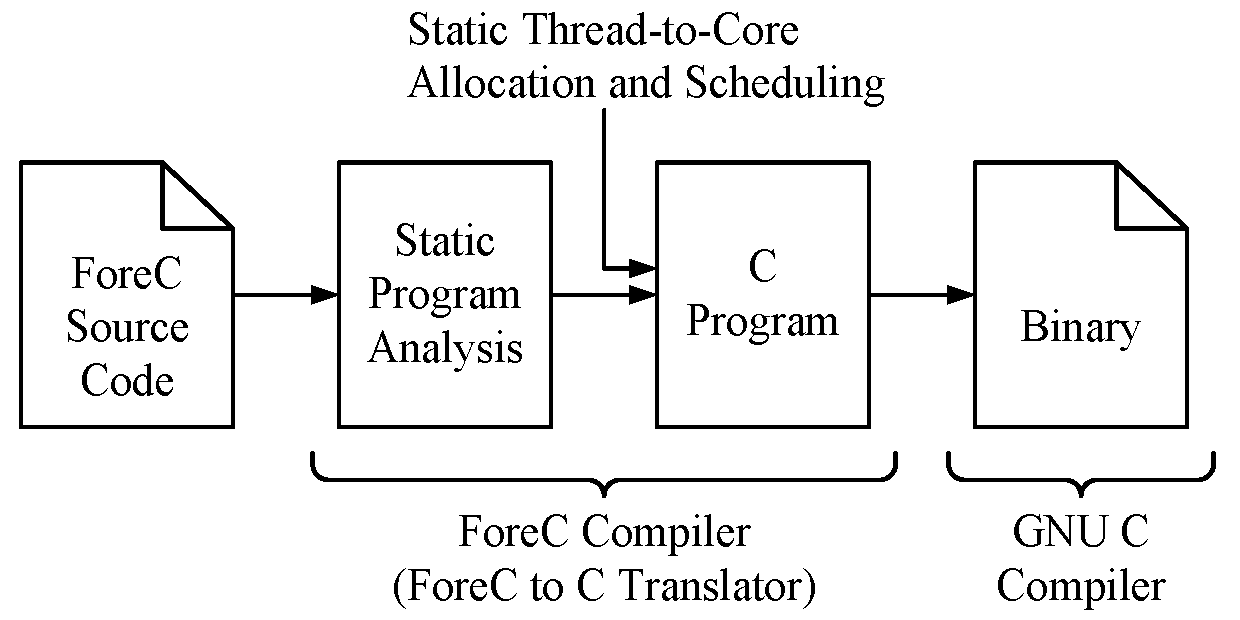
\includegraphics[width=0.6\columnwidth]{images/compilation_embedded_overview.pdf}

	\caption{Overview of compiling ForeC programs.}
	\label{fig:forec_compiling:overview}
\end{figure}

\begin{figure}
	\centering

	\begin{minipage}{0.47\columnwidth}
		\subfloat[Example ForeC program.]{
			\lstinputlisting[style=full]{./code/forec_compiling/example.forec}
			\label{fig:forec_compiling:example:forec}	
		}
	\end{minipage}
	\hspace{1cm}
	\begin{minipage}{0.25\columnwidth}
		\centering
		\subfloat[Total order.]{
			
\includegraphics[width=0.6\columnwidth]{total_order}
			\label{fig:forec_compiling:total_order}	
		}
		\vspace{1cm}
		\subfloat[Thread allocation.]{
			\begin{tabular}{c c c}
				{\bf Core 1}	&	& {\bf Core 2}	\\
				\cline{1-1}\cline{3-3}
				main			&	& tB			\\
				tA				&	& tD			\\
				tC				&	&				\\
			\end{tabular}
			\label{fig:forec_compiling:schedule}	
		}
	\end{minipage}
	
	\vfill
	
	\subfloat[Possible execution trace of the compiled program.]{
			
\includegraphics[width=0.65\columnwidth]{forec_timing}
			\label{fig:forec_compiling:timing}	
	}
	\caption{Example ForeC program to be compiled.}
\end{figure}


\subsection{Static Thread Scheduling}
\label{sec:forec_compiling:scheduling}
This section deals exclusively with ForeC threads.
We illustrate the static thread scheduling with the 
example of Figure~\ref{fig:forec_compiling:example:forec}. 
The programmer statically allocates the
threads to the cores and passes the allocations into the
compiler. The scheduling is \emph{static} and \emph{non-preemptive}
(cooperative). Thus, threads execute without interruption
until they reach a \emph{context-switching point}: a \verb$par$ or
\verb$pause$ statement, or the end of their body. 
The semantics of shared variables (see Section~\ref{sec:forec:shared_variables}) 
ensures that threads execute their local ticks in isolation, e.g., 
independently of their siblings or their parent's siblings.
The compiler defines a total order for all the threads.
The total order is based on the depth-first traversal of the thread hierarchy.
Figure~\ref{fig:forec_compiling:total_order} depicts the thread
hierarchy of the ForeC program from Figure~\ref{fig:forec_compiling:example:forec},
where numbers indicate the total order. A lower number
means higher execution priority.
Figure~\ref{fig:forec_compiling:schedule} shows a possible
thread allocation chosen by the programmer for two cores, in their thread scheduling
order. When a thread reaches a \verb$par$ statement, its 
child threads are forked for execution on their allocated
cores. The core that executes the parent thread is
called the \emph{master} core.
The cores that execute the child threads are called 
the \emph{slave} cores. Depending 
on the thread allocations, a core could be the master core 
of one thread and be the slave core of another 
thread. For the \verb$par$ statement on 
line~\ref{code:forec_compiling:forec_par1} of 
Figure~\ref{fig:forec_compiling:example:forec},
core 1 is the master core and core 2 is the slave core.

Based on the the thread allocation and scheduling order shown in 
Figure~\ref{fig:forec_compiling:schedule}, 
Figure~\ref{fig:forec_compiling:timing} is a possible execution trace.
The trace for both cores (``Core~1'' and ``Core~2'') 
progresses downwards from the top of Figure~\ref{fig:forec_compiling:timing}.
Thread executions are shown as white segments in the 
trace and each one has the thread's name and the executed 
lines of code from Figure~\ref{fig:forec_compiling:example:forec}.
The compiler generates \emph{synchronization routines} to 
manage the thread executions on the master and slave
cores. These routines are shown as shaded segments in the 
trace and each one has the routine's name. 
The names are prefixed with ``\verb$m$'' or ``\verb$s$'' 
to identify whether a routine is for a master or slave 
core, respectively. The names are suffixed with an integer 
to identify the unique id assigned to each \texttt{par} (with a 
depth-first traversal of the thread hierarchy starting from the root).
For example, the \verb$mFork1$, 
\verb$sFork1$, \verb$mJoin1$, and \verb$sJoin1$ routines in 
Figure~\ref{fig:forec_compiling:timing} all
manage the threads forked by thread \verb$main$. 
Table~\ref{table:forec_compiling:routines}
summarizes the behavior of the routines. The 
\verb$mFork$ and \verb$sFork$ routines manage
the forking of child threads (Section~\ref{sec:forec_compiling:par}). The 
\verb$mJoin$ and \verb$sJoin$ routines manage
the joining of child threads (Section~\ref{sec:forec_compiling:par}). 
The \verb$mSync$ and \verb$sSync$ routines manage
the global tick synchronization of all the cores (Section~\ref{sec:forec_compiling:sync}).
In Figure~\ref{fig:forec_compiling:timing}, the synchronization 
between the routines are shown as arrows marked 
with the information that is sent. The information is an 
integer value that encodes the following execution states 
of a thread: 0 (\verb$TERM$) for thread termination, 1 and 
greater for the unique id of the \texttt{par} statement that 
is executing, and -1 
(\verb$OTHER$) for executing a \verb$pause$ statement
or for not executing a \verb$par$ statement.

\begin{table}
	\def\arraystretch{1.3}
	\tbl{Summary of the synchronization routines.\label{table:forec_compiling:routines}}{
		\begin{tabular}{| p{\columnwidth} |}
			\hline
			\texttt{mFork}:	Uses a non-blocking send to notify the slave 
							cores whether or not the parent thread has forked.		\\ 
			\texttt{sFork}:	Blocks until it receives whether or not the parent 
							thread has forked.										\\ \hline
			\texttt{mJoin}:	Blocks until it receives whether the child threads 
							on other cores have terminated. Then, it notifies 
							the slave cores whether the parent thread has resumed.	\\ 
			\texttt{sJoin}:	Uses a non-blocking send to notify the master core 
							whether or not its child threads have terminated. Then, 
							it blocks until it receives whether the parent thread 
							has resumed.											\\ \hline
			\texttt{mSync}:	Synchronizes with all the cores, performs the
							housekeeping tasks, and then synchronizes with all the 
							cores again to start the next global tick.				\\ 
			\texttt{sSync}:	Synchronizes with all the cores and waits for the 
							next synchronization to start the next global tick.		\\ \hline
			\texttt{mAbort} and \texttt{sAbort}:	Evaluates the preemption 
							condition of an \texttt{abort}.							\\
			\hline
		\end{tabular}
	}
\end{table}

\begin{figure}
	\centering

	\begin{minipage}{0.4\columnwidth}
%		\subfloat[node.h]{
			\lstinputlisting[style=full]{./code/forec_compiling/linkednode.c}
%			\label{fig:forec_compiling:linkednode}
%		}
	\end{minipage}
%	\hspace{1cm}
%	\begin{minipage}{0.3\columnwidth}
%		\subfloat[insert(n1,n2)]{
%			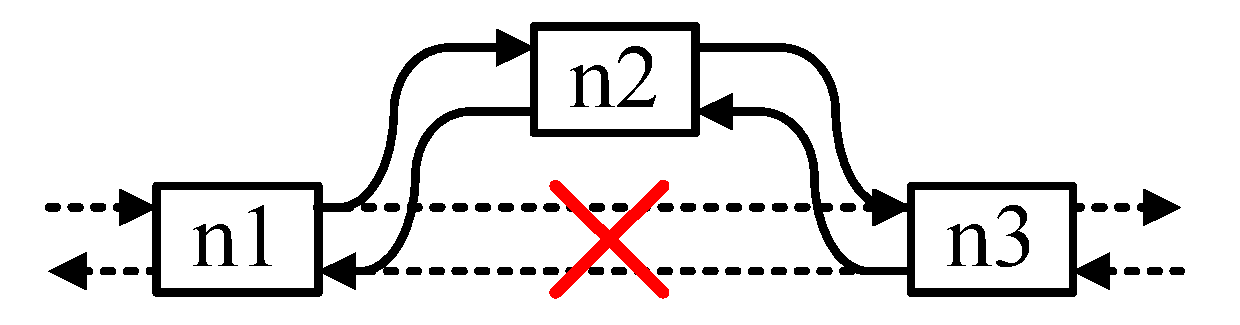
\includegraphics[width=\columnwidth]{images/list_insert.pdf}
%			\label{fig:forec_compiling:list_insert}	
%		}
%		\vspace{1cm}
%		\subfloat[remove(n2)]{
%			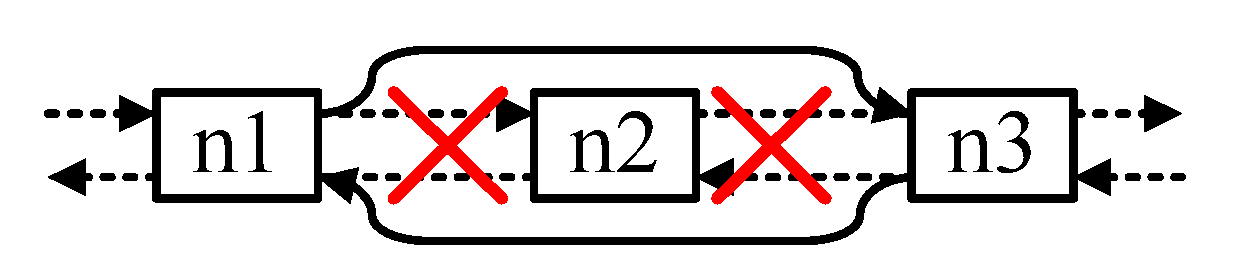
\includegraphics[width=\columnwidth]{images/list_remove.pdf}
%			\label{fig:forec_compiling:list_remove}	
%		}
%	\end{minipage}

	\caption{Definition of a linked list node and its operations in \texttt{node.h}.}
	\label{fig:forec_compiling:linkednode}
\end{figure}

The threads and synchronization routines are statically 
scheduled on each core with \emph{doubly linked lists}. 
Each node (defined in Figure~\ref{fig:forec_compiling:linkednode}) 
of a linked list represents a thread or a synchronization
routine and stores its continuation point (\verb$pc$) and
the links to its adjacent nodes (\verb$prev$ and
\verb$next$). A node's \verb$pc$ is initially set to the
start of the thread or routine's body. Each core starts its
scheduling by jumping to the \verb$pc$ of its first node.
When a context-switching point is reached during the
execution of a thread or routine, a jump is made to the
\verb$pc$ of the next node. A core will only execute the
threads and routines in its linked list. Thus, inserting or
removing a thread or routine from the list controls whether
it is included or excluded, respectively, from execution. 
The remainder of this section describes how a ForeC program is
compiled into a C program and how the linked lists are created
and used to implement the ForeC semantics. 


\subsection{Structure of the Generated Program}
Figure~\ref{fig:forec_compiling:example:c1} 
shows a simplified version of the C program generated for the
ForeC program in Figure~\ref{fig:forec_compiling:example:forec}. 
All line numbers in section refer to Figure~\ref{fig:forec_compiling:example:c1}.
The generated C program contains:
\begin{itemize} 
	\item The global declarations and functions from the ForeC program
		  (lines~\ref{code:forec_compiling:example_user1}--\ref{code:forec_compiling:example_user2}).
	\item The global declarations for storing the execution states of the threads and implementing the shared variables 
		  (lines~\ref{code:forec_compiling:example_scheduling1}--\ref{code:forec_compiling:example_copies}).
	\item The \verb$main$ function (line~\ref{code:forec_compiling:example_forecmain})
		  with the bootup routine (lines~\ref{code:forec_compiling:example_scheduler1}--\ref{code:forec_compiling:example_direct2}),
		  the synchronization routines 
		  (lines~\ref{code:forec_compiling:example_mFork1}--\ref{code:forec_compiling:example_scheduler2}), 
		  and the threads (lines~\ref{code:forec_compiling:example_threads1}--\ref{code:forec_compiling:example_threads2}). 
\end{itemize}
Although the scheduling routines dominate the generated code 
in Figure~\ref{fig:forec_compiling:example:c1}, their code remains constant 
whatever the size of the user-defined threads (which could be arbitrarily large).
When the cores enter the \verb$main$ function, they execute
the bootup routine to initialize their linked lists. First, 
a node is created for each thread and each synchronization routine
(lines~\ref{code:forec_compiling:example_scheduling3}--\ref{code:forec_compiling:example_scheduling4}). 
Second, the nodes are linked together to create the initial
linked list for each core (lines~\ref{code:forec_compiling:example_direct1}--\ref{code:forec_compiling:example_direct2}).
These initial lists are illustrated in the second row of 
Table~\ref{tab:forec_compiling:lists}. The threads and 
routines are inlined into the \verb$main$ function because fast
context-switching is implemented by jumping between C labels
with GNU's computed \verb$goto$ extension. Jumping with \verb$goto$ 
is restricted to C labels located in the same function scope. To avoid the need to 
create stacks for each thread to maintain their local variables, 
the local variables are given unique names and hoisted up to the 
global scope (e.g., \verb$tC$'s local variable
\verb$a$ on line~\ref{code:forec_compiling:example_a}). 
However, functions executed on the same core will
share the same stack space. To avoid stack corruption, all the
functions must execute atomically, i.e., without interruption. 

\begin{figure}
	\centering

	\lstinputlisting[style=fulltight,multicols=2,frame=tlr,lastline=120]{./code/forec_compiling/example.c}

	\caption{Example of the C program generated for Figure~\ref{fig:forec_compiling:example:forec}.}
	\label{fig:forec_compiling:example:c1}
\end{figure}

\begin{figure}
	\ContinuedFloat 
	\centering

	\lstinputlisting[style=fulltight,multicols=2,frame=lrb,firstline=121,firstnumber=121]{./code/forec_compiling/example.c}

	\caption{(Continued.) Example of the C program generated for Figure~\ref{fig:forec_compiling:example:forec}.}
	\label{fig:forec_compiling:example:c2}
\end{figure}


\subsection{The \texttt{par} Statement}
\label{sec:forec_compiling:par}
The execution of a ForeC program starts with its \verb$main$
thread. The slave cores must wait for their allocated
threads to be forked. \emph{The global tick in which threads fork and
join can only be determined at runtime.} Hence, before a core
executes a thread, it must check that no other higher
priority thread allocated to it will be forked. Otherwise,
the higher priority thread must be executed first. This is
achieved by scheduling an \verb$mFork$ routine after a
parent thread completes its local tick. It uses a
\emph{non-blocking send} to notify the slave cores whether
or not the parent thread has forked. Thus, a slave core uses
an \verb$sFork$ routine to \emph{block} until it receives
whether or not the parent thread has forked. To ensure
correct scheduling order, the \verb$sFork$ routine has the
same execution priority as the parent thread. When a fork
does occur, the \verb$mFork$ and \verb$sFork$ routines
instruct their cores to suspend the parent thread and to
schedule the child thread. In the first 
global tick of Figure~\ref{fig:forec_compiling:timing},
\verb$mFork1$ notifies \verb$sFork1$ that thread \verb$main$
has not forked (\verb$OTHER$ is sent). In the second global tick, 
\verb$mFork1$ notifies \verb$sFork1$ that thread \verb$main$
has forked (\verb$1$ is sent).

Before a core executes a parent thread that was suspended by
a fork, it must check that all of its child threads have
terminated. This is achieved by scheduling an \verb$mJoin$
routine after the child threads on the master core have
completed their respective local ticks. It \emph{blocks}
until it receives whether or not the child threads on the
slave cores have terminated. When all child threads have
terminated, the \verb$mJoin$ routine instructs the master
core to resume the parent thread. Thus, each slave core
schedules an \verb$sJoin$ routine after its child threads
complete their respective local ticks. It uses a
\emph{non-blocking send} to notify the master core whether
or not the child threads on the slave core have terminated. 
In the second and third global ticks of 
Figure~\ref{fig:forec_compiling:timing}, \verb$sJoin1$
notifies \verb$mJoin1$ that thread \verb$tB$ has 
terminated (\verb$TERM$ is sent).

\begin{table}
	\centering
	\tbl{Core 1 and 2's initial lists and subsequent lists when threads fork.\label{tab:forec_compiling:lists}}{
		\begin{tabular}{| c | l |}
			\hline
			\textbf{Execution Point}		& \multicolumn{1}{c|}{\textbf{Linked Lists}}														\\
			\hline
			When the program starts			& \raisebox{0.15cm}{\textbf{Core 1:}} 
\includegraphics[height=0.55cm]{images/list_m1.pdf}			\\
											& \raisebox{0.15cm}{\textbf{Core 2:}} 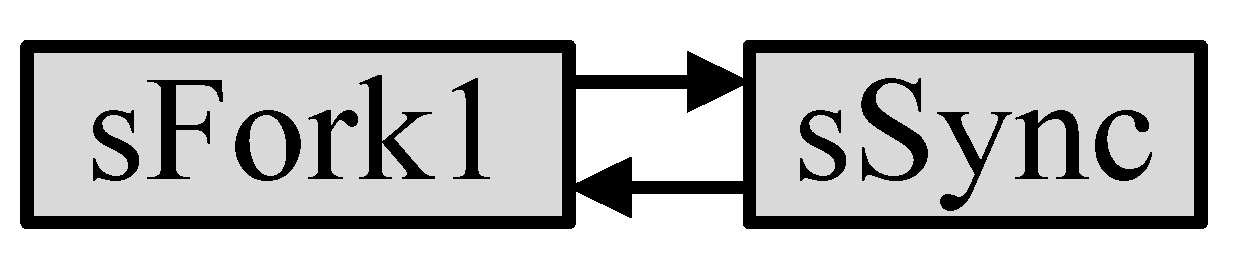
\includegraphics[height=0.55cm]{images/list_s1.pdf}			\\ \hline
			When \texttt{main} \par forks (id = 1)	& \raisebox{0.15cm}{\textbf{Core 1:}} 
\includegraphics[height=0.50cm]{images/list_m2.pdf}	\\
											& \raisebox{0.15cm}{\textbf{Core 2:}} 
\includegraphics[height=0.49cm]{images/list_s2.pdf}			\\ \hline
			When \texttt{tB} \par forks (id = 2)	& \raisebox{0.15cm}{\textbf{Core 1:}} 
\includegraphics[height=0.49cm]{images/list_m3.pdf}	\\
											& \raisebox{0.15cm}{\textbf{Core 2:}} 
\includegraphics[height=0.50cm]{images/list_s3.pdf}			\\
			\hline
		\end{tabular}
	}
\end{table}

We now describe the C code that is generated for each
\verb$par$ statement and how the synchronization routines
are incorporated into the linked lists. 
The last two rows of Table~\ref{tab:forec_compiling:lists} 
visualizes core 1 and~2's linked 
lists when threads \verb$main$ and \verb$tB$ fork 
(lines~\ref{code:forec_compiling:example_par1} and 
\ref{code:forec_compiling:example_par2} respectively). 
Each \verb$par$ 
statement is assigned a unique positive integer 
\verb$id$ by the compiler.
Lines~\ref{code:forec_compiling:example_par1}--\ref{code:forec_compiling:example_join1}
in Figure~\ref{fig:forec_compiling:example:c1} is an 
example of the C code that is generated for a \verb$par$ 
statement. Line~\ref{code:forec_compiling:example_state}
sets the parent thread's execution state to \verb$id$
and sets the 
parent thread's \verb$pc$ to be immediately after the 
\verb$par$ statement. Line~\ref{code:forec_compiling:example_switch}
is a context-switch to the parent thread's 
\verb$mFork$ routine. 
Lines~\ref{code:forec_compiling:example_mFork1}--\ref{code:forec_compiling:example_mFork1_end}
is an example of the C code that is generated for an 
\verb$mFork$ routine. Line~\ref{code:forec_compiling:example_send1}
sends the parent thread's execute state to the slave cores.
If the parent thread has forked, then 
lines~\ref{code:forec_compiling:example_mAbort1_insert}--\ref{code:forec_compiling:example_mFork1_goto1}
insert the allocated child threads and an \verb$mJoin$ 
routine into the linked list. The parent thread and 
\verb$mFork$ routine are removed from the linked list.
If a child thread can fork its own threads,
then further \verb$mFork$ and \verb$sFork$ routines need to be
inserted into the linked lists. This ensures that the nested
threads can be forked. 
The end of line~\ref{code:forec_compiling:example_mFork1_goto1} is
a context-switch to the first node that was inserted. 
Otherwise, if the parent thread has not forked, then
line~\ref{code:forec_compiling:example_mFork1_goto2} is
a context-switch to the next node in sequence.

Recall that the slave cores have an \verb$sFork$
routine in their initial linked list. 
Lines~\ref{code:forec_compiling:example_sFork1}--\ref{code:forec_compiling:example_sFork1_end}
is an example of the C code that is generated for an \verb$sFork$
routine. Line~\ref{code:forec_compiling:example_receive1}
blocks until it receives whether the parent thread has
forked. If the parent thread has forked, then 
line~\ref{code:forec_compiling:example_sAbort1_insert}
inserts the allocated child threads and an \verb$sJoin$
routine into the linked list. The \verb$sFork$ routine 
is removed from the linked list. The end of 
line~\ref{code:forec_compiling:example_sFork1_goto1} is
a context-switch to the first node that was inserted.
Otherwise, if the parent thread has not forked, then
line~\ref{code:forec_compiling:example_sFork1_goto2} is
a context-switch to the next node in sequence.

Lines~\ref{code:forec_compiling:example_term1}--\ref{code:forec_compiling:example_term4} 
in Figure~\ref{fig:forec_compiling:example:c1} is an example 
of the C code that is generated for the end of a child 
thread to handle thread termination. 
Line~\ref{code:forec_compiling:example_term2} sets the thread's
execution state to \verb$TERM$. 
Line~\ref{code:forec_compiling:example_term3} removes the thread
from the linked list. 
Line~\ref{code:forec_compiling:example_term4} is a context-switch 
to the next node in sequence.
Lines~\ref{code:forec_compiling:example_mJoin1}--\ref{code:forec_compiling:example_mJoin1_end} 
is an example of the C code that is generated for an 
\verb$mJoin$ routine. 
Line~\ref{code:forec_compiling:example_receive2} blocks 
until it receives the execution state of each child thread.
If all the child threads have terminated, then 
line~\ref{code:forec_compiling:example_receive2_term1}
sets the execution state of the parent thread to \verb$OTHER$
and sends that state to the slave cores. 
Lines~\ref{code:forec_compiling:example_receive2_term2}--\ref{code:forec_compiling:example_receive2_term3}
insert the parent thread back into the linked list and 
removes the nodes associated with the \verb$par$ statement. 
This is followed by a context-switch to the parent thread.
Otherwise, if some child threads have not terminated, then
line~\ref{code:forec_compiling:example_receive2_term4} is 
is a context-switch to the next node in sequence.
Lines~\ref{code:forec_compiling:example_sJoin1}--\ref{code:forec_compiling:example_sJoin1_end}
is an example of the C code that is generated for an 
\verb$sJoin$ routine. 
Line~\ref{code:forec_compiling:example_send2} sends the 
execution state of each child thread to the master core.
Line~\ref{code:forec_compiling:example_sJoin1_receive}
blocks until it receives whether the parent thread has
been resumed. If the parent thread has been resumed, then
line~\ref{code:forec_compiling:example_sJoin1_term} removes
the \verb$sJoin$ routine from the linked list. 
Line~\ref{code:forec_compiling:example_sJoin1_goto} is a 
context-switch to the next node in sequence.


\subsection{The \texttt{pause} Statement}
The \verb$pause$ statement is a context-switching point and 
lines~\ref{code:forec_compiling:example_pause1}--\ref{code:forec_compiling:example_pause1_end} 
in Figure~\ref{fig:forec_compiling:example:c1}
is an example of the C code that is generated.
Line~\ref{code:forec_compiling:example_pause2} sets the
current thread's \verb$pc$ to be immediately after
the \verb$pause$ statement.
Line~\ref{code:forec_compiling:example_pause3} is a 
context-switch to the next node in sequence.
In the next global tick, execution will resume from statement 
immediately after the \verb$pause$ statement.


\subsection{Shared Variables}
Shared variables are hoisted up to the program's global 
scope to allow all cores to access them (e.g., 
line~\ref{code:forec_compiling:example_user1} in 
Figure~\ref{fig:forec_compiling:example:c1}). The copies of 
shared variables are implemented as unique global variables 
(e.g., line~\ref{code:forec_compiling:example_copies}) to
allow them to be combined on different cores. In each 
thread, all shared variable 
accesses are replaced by accesses to their copies
(e.g., lines~\ref{code:forec_compiling:example_x_main} and 
\ref{code:forec_compiling:example_x_tA}). 
The shared variables are copied at the start of each 
local tick, i.e., start of each 
thread body, and after each \verb$pause$ 
and \verb$par$ statement. For example, the shared variable
\verb$x$ on line~\ref{code:forec_compiling:example_user1}
is copied by thread \verb$main$ on 
lines~\ref{code:forec_compiling:example_copy1}, 
\ref{code:forec_compiling:example_copy2} and 
\ref{code:forec_compiling:example_copy3}.
As defined by the (\ref{forec:par-4}), (\ref{forec:par-5}), 
(\ref{forec:par-6}), and (\ref{forec:par-7}) semantic rules 
given in Section~\ref{sec:forec_semantics:sos}, 
the \verb$par$ statement is responsible for combining the copies
of shared variables. More precisely, when the child threads
of a \verb$par$ statement complete their respective local ticks,
their copies of shared variables are combined. The combined
result is assigned to their parent thread. This combine process
is implemented by the \verb$mJoin$ routine (e.g., 
line~\ref{code:forec_compiling:example_combine2}) because it 
waits for the child threads to complete their respective local 
ticks. The final values of the shared variables are computed 
by the \verb$mJoin$ routine of thread \verb$main$.


\subsection{The \texttt{abort} Statement}
We begin by describing the C code that is generated 
for an \verb$abort$ that does not have the optional 
\verb$immediate$ or \verb$weak$ keywords. 
Conditional jumps, using the preemption condition, 
are inserted after each \verb$pause$ statement in the 
\verb$abort$ body. For example, 
lines~\ref{code:forec_compiling:example_abort1}--\ref{code:forec_compiling:example_abort3} 
in Figure~\ref{fig:forec_compiling:example:c1} is an 
\verb$abort$ and a conditional jump is inserted on 
line~\ref{code:forec_compiling:example_abort2} 
after the \verb$pause$ statement.
The preemption condition \verb$x>1$ is used 
in the conditional jump. If the preemption 
condition evaluates to \emph{true}, a jump is
made to the statement immediately after the
\verb$abort$ (e.g., line~\ref{code:forec_compiling:example_abort4}).
If a \verb$par$ statement is inside
the \verb$abort$ body, then the preemption condition must be
evaluated before the threads can execute. For example, 
in the third global tick of Figure~\ref{fig:forec_compiling:timing},
the cores use the \verb$mAbort$ and \verb$sAbort$ routines to evaluate
the preemption condition on 
line~\ref{code:forec_compiling:forec_preemption} of 
Figure~\ref{fig:forec_compiling:example:forec}. It is safe to 
evaluate the preemption conditions in parallel because 
they are side-effect free by definition (Section~\ref{sec:forec:preemption}).
Thus, when a fork occurs, an \verb$Abort$ routine 
is inserted before the child threads in the linked lists. 
For a master core, 
lines~\ref{code:forec_compiling:example_mAbort1}--\ref{code:forec_compiling:example_mAbort1_end} 
in Figure~\ref{fig:forec_compiling:example:c1} 
is an example of the C code that is generated for an 
\verb$mAbort$ routine. 
Line~\ref{code:forec_compiling:example_mAbort1_1} 
evaluates the preemption condition. If it evaluates
to \emph{true}, then line~\ref{code:forec_compiling:example_mAbort1_2}
removes the nodes associated with the \verb$par$ statement.
Line~\ref{code:forec_compiling:example_mAbort1_3} sets the 
parent thread's \verb$pc$ to be immediately after the
\verb$abort$ statement and context-switches to the parent
thread. Otherwise, if the preemption condition evaluates
to \emph{false}, then line~\ref{code:forec_compiling:example_mAbort1_4}
is a context-switch to the next node in sequence.
For a slave core, 
lines~\ref{code:forec_compiling:example_sAbort1}--\ref{code:forec_compiling:example_sAbort1_end} 
is an example of the C code that is generated for an \verb$sAbort$
routine and is similar to that of an \verb$mAbort$.
Line~\ref{code:forec_compiling:example_sAbort1_1}
evaluates the preemption condition. If it evaluates
to \emph{true}, then line~\ref{code:forec_compiling:example_sAbort1_2}
removes the nodes associated with the \verb$par$ statement.
Line~\ref{code:forec_compiling:example_sAbort1_3} is a 
context-switch to the next node in sequence. Otherwise, 
if the preemption condition evaluates
to \emph{false}, then line~\ref{code:forec_compiling:example_sAbort1_4}
is a context-switch to the next node in sequence.

\begin{figure}
	\centering

	\begin{minipage}{0.28\columnwidth}
		\vspace{0.67cm}
		\subfloat[Immediate and strong \texttt{abort}.]{
			\lstinputlisting[style=fulltight,numbers=none]{./code/forec_compiling/immediate_abort.c}
			\label{fig:forec_compiling:immediate_abort}	
		}
	\end{minipage}
	\hfill
	\begin{minipage}{0.25\columnwidth}
		\vspace{0.67cm}
		\subfloat[Non-immediate and weak \texttt{abort}.]{
			\lstinputlisting[style=fulltight,numbers=none]{./code/forec_compiling/weak_abort.c}
			\label{fig:forec_compiling:weak_abort}	
		}
	\end{minipage}
	\hfill
	\begin{minipage}{0.31\columnwidth}
		\subfloat[Immediate and weak \texttt{abort}.]{
			\lstinputlisting[style=fulltight,numbers=none]{./code/forec_compiling/immediate_weak_abort.c}
			\label{fig:forec_compiling:immediate_weak_abort}	
		}
	\end{minipage}

	\caption{C code for the immediate and weak variants of the \texttt{abort} on 
			lines~\ref{code:forec_compiling:example_abort1}--\ref{code:forec_compiling:example_abort3} 
			of Figure~\ref{fig:forec_compiling:example:c1}.}
\end{figure}

The optional \verb$immediate$ keyword allows the preemption
condition to be evaluated before the \verb$abort$ body is
executed for the first time. Thus, an additional conditional 
jump, using the preemption condition, is inserted at the 
start of the \verb$abort$ body. Figure~\ref{fig:forec_compiling:immediate_abort}
is an example of the C code that would be generated if the \verb$abort$ on 
lines~\ref{code:forec_compiling:example_abort1}--\ref{code:forec_compiling:example_abort3} 
in Figure~\ref{fig:forec_compiling:example:c1} was 
an immediate \verb$abort$.
The optional \verb$weak$ keyword delays the jumping to the 
end of the \verb$abort$ body when the preemption condition
evaluates to \emph{true}. Thus, the conditional jump is separated
into two parts: (1) the evaluation of the preemption condition
and (2) the resulting jump. The evaluation is inserted directly 
after each \verb$pause$ statement and the jump is inserted 
directly before each \verb$pause$ statement. If a \verb$par$ 
statement is inside the weak \verb$abort$, then the 
\verb$mAbort$ and \verb$sAbort$ routines are inserted after 
the child threads in the linked lists. 
Figure~\ref{fig:forec_compiling:weak_abort}
is an example of the C code that would be generated if the \verb$abort$ on 
lines~\ref{code:forec_compiling:example_abort1}--\ref{code:forec_compiling:example_abort3} 
in Figure~\ref{fig:forec_compiling:example:c1} was 
a weak \verb$abort$. 
Figure~\ref{fig:forec_compiling:immediate_weak_abort} 
is an example of the C code generated if it was an 
immediate and weak \verb$abort$.


\subsection{Global Tick Synchronization}
\label{sec:forec_compiling:sync} 
The notion of a global tick is preserved by ending each linked 
list with a \verb$Sync$ routine that implements \emph{barrier synchronization}. 
This synchronization is shown at the end of each global tick in 
Figure~\ref{fig:forec_compiling:timing}.
For the master core that executes the \verb$main$ thread, 
lines~\ref{code:forec_compiling:example_mSync}--\ref{code:forec_compiling:example_mSync_end} 
is an example of the C code that is generated for 
an \verb$mSync$ routine.
Line~\ref{code:forec_compiling:example_mSync_1} is a 
barrier synchronization for the end of the tick. 
Line~\ref{code:forec_compiling:example_mSync_2} 
performs the following housekeeping tasks: finalizing the
values of the shared variables, emitting outputs, and
sampling inputs.
Line~\ref{code:forec_compiling:example_mSync_3} is 
a barrier synchronization to signal the start of the 
next global tick. 
Line~\ref{code:forec_compiling:example_mSync_4} is a
context-switch to the first node in the linked list.
For the remaining slave cores, 
lines~\ref{code:forec_compiling:example_sSync}--\ref{code:forec_compiling:example_scheduler2}
is an example of the C code that is generated for an
\verb$sSync$ routine.
Line~\ref{code:forec_compiling:example_sSync_1} are
barrier synchronizations for the end of the tick
and the start of the next tick. This is followed by 
a context-switch to the first node in the linked list.

%\subsection{Optimizations}
%Inlined nesting of \verb$par$ statements (each nested 
%\verb$par$ statement is not in sequence with any other 
%statement): Fork and join all the nested threads together.
%
%Shared variable that does not need a combine function: Assign
%the writer's copy directly to the shared variable.
%
%Shared variable that is only read by a thread: Apart from the
%thread's first local tick (where the parent's copy is read), 
%the shared variable can be read in subsequent local ticks.


\subsection{Generating Programs for Execution on Operating Systems}
\label{sec:forec_compiling:posix}
This section describes how the ForeC compiler is extended to
generate executable code for operating systems. 
To utilize multiple cores in a system, a program
must create multiple threads that the operating system can 
schedule. We modify the ForeC compiler to generate a 
Pthread~\cite{multiprocessor_pthreads} for each core in the system. Each
Pthread is responsible for executing the ForeC threads
statically allocated to the same core, as shown in
Figure~\ref{fig:forec_compiling:os}. In effect, a fixed pool of
Pthreads executes the ForeC threads and the cost of creating
each Pthread is only incurred once. Although the
Pthreads will be dynamically scheduled by the operating
system, the original ForeC threads will still follow their
static schedule. Finally, the generated 
Pthreads program is compiled with a GNU C compiler.

\begin{figure}
	\centering

	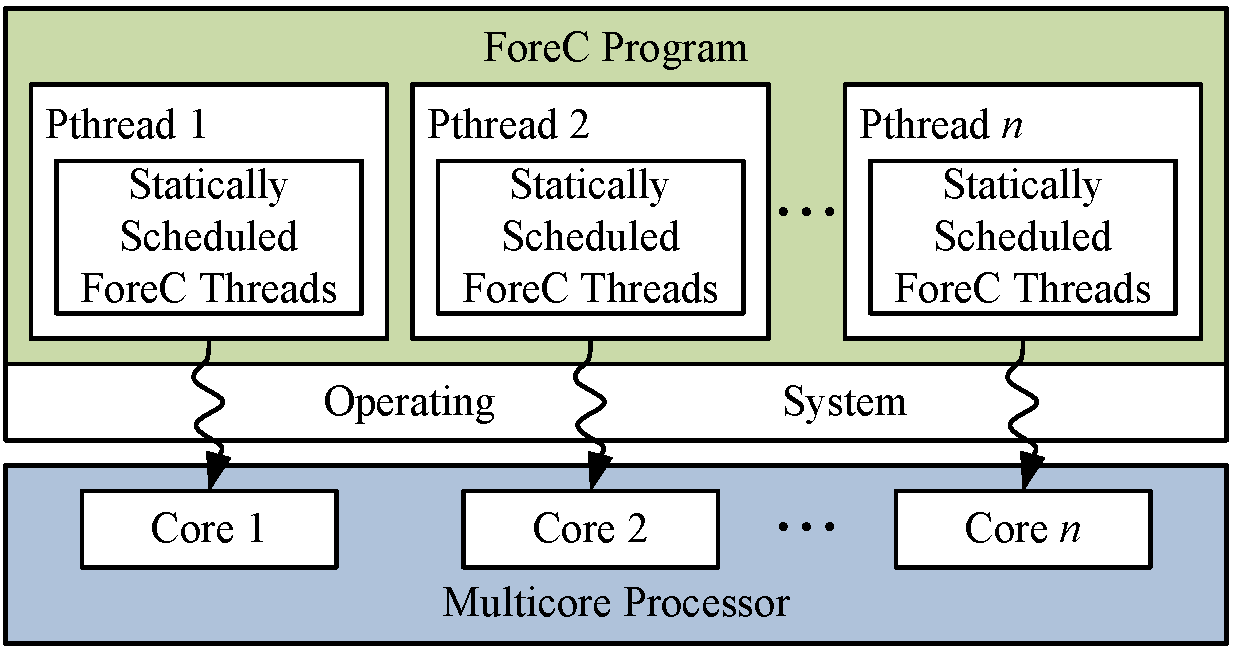
\includegraphics[width=0.7\columnwidth]{images/compilation_os.pdf}

	\caption{Using Pthreads to adapt the generated code for multi-cores.}
	\label{fig:forec_compiling:os}
\end{figure}

\begin{figure}
	\centering

	\begin{minipage}{0.85\columnwidth}
		\lstinputlisting[style=fulltight]{./code/forec_compiling/example_desktop.c}
	\end{minipage}

	\caption{Example Pthreads program.}
	\label{fig:forec_compiling:example:c:desktop}
\end{figure}

For the ForeC program of Figure~\ref{fig:forec_compiling:example:forec}, 
Figure~\ref{fig:forec_compiling:example:c:desktop} is a 
simplified extract of the generated Pthreads program. 
In addition to the global declarations shown in 
Figure~\ref{fig:forec_compiling:example:c1}, there are
now Pthreads-related declarations
(lines~\ref{code:forec_compiling:example:desktop:pthread1}--\ref{code:forec_compiling:example:desktop:pthread2}) 
and a new \verb$main$ function for creating the 
Pthreads~(line~\ref{code:forec_compiling:example:desktop:main}).
The original \verb$main$ function from Figure~\ref{fig:forec_compiling:example:c1} 
(line~\ref{code:forec_compiling:example_forecmain}) 
is renamed as \verb$forecMain$ (line~\ref{code:forec_compiling:example:desktop:forecmain}).
When the operating system executes the \verb$main$
function, the Pthreads start executing the 
\verb$forecMain$ function and, hence, the statically 
allocated ForeC threads.


\subsection{Discussion}
This section has presented the compilation of ForeC
programs for direct execution on parallel hardware architectures. 
The compilation is syntax-driven and templates are
used to generate code for each ForeC construct. Light-weight
synchronization routines are generated to manage the forking
and joining of threads across the cores. The use of linked
lists to manage the scheduling of threads and routines is
inspired by that of the Columbia Esterel Compiler~\cite{timed_cec}.
The code generation
is structural, meaning that a nesting of ForeC constructs is
compiled into a nesting of each construct's generated code.
The advantages with our static scheduling approach include: 
(1) a light-weight scheduling of ForeC threads, and
(2) analysis is easier because all scheduling decisions are 
known beforehand.
However, the disadvantages include:
(1) the inability to dynamically load balance the ForeC threads 
to utilize the idle cores, and
(2) the need to recompile the program to target a different 
number of cores.
Memory fences in C (e.g.,
\texttt{atomic\_thread\_fence}~\cite{programming_languages_c11}) 
are not used to implement the semantics of shared
variables because (1) the reading of inputs and the writing
of outputs for global tick synchronisation already requires
barrier synchronization among the cores, making memory fences 
redundant for the finalizing shared variables, and (2) memory fences
on shared variables are unable to isolate the accesses of
one thread from the accesses of another thread, which is needed
during each local tick.


For future work, the dynamic scheduling of 
ForeC threads can be developed to improve the average-case 
performance on desktop computers. 
In future versions of the compiler, we also wish to implement 
proper thread stacks to allow the execution of functions 
that pause.

The distribution of traditional synchronous programs over multiple 
processors is not new~\cite{distributed_reactive_systems_survey,distributed_synchronous_dependency_driven,distributed_reactive_systems_automatic,wcrt_esterel_multicores,YuanYR11,timed_esterel_distribution_emperor,timed_multiclock_multithreaded}.
It is motivated by the desire to execute computations closer
to their inputs and outputs, which may be distributed over a
geographical area. Unfortunately, the use of signals for
instantaneous communication makes compilation notoriously
difficult. First, \emph{causality analysis}~\cite{timed_compiling_esterel} 
is needed to ensure that the presence or absence of all signals
can be determined exactly in each global tick. Second, the compiler 
must generate code for resolving signal statuses at runtime.
A common approach is to compile away the parallelism and to generate
a sequential program~\cite{timed_cec,timed_compiling_esterel}.
Third, the sequential program is partitioned into subprograms 
and distributed to execute on their allocated processors. 
Desynchronization techniques~\cite{BenvenisteCG00,GiraultNP06,distributed_synchronous_desynchronize_modes} 
can be used when the processors execute and communicate at different speeds. 
SynDEx~\cite{distributed_synchronous_semantics_preserving} is 
a tool that automatically distributes synchronous programs and 
considers the cost of communication between the processors.
In contrast, ForeC is significantly easier to compile because thread
communication is delayed with shared variables 
(Section~\ref{sec:forec:shared_variables}). Causality analysis
is not required and ForeC threads can be distributed directly
to the available cores. The parallelism specified by
the programmer is preserved by the ForeC compiler and a
sequential intermediate code is not required.

With the advent of multi-cores, the distribution of
synchronous programs is motivated by the desire to improve
their execution performance. The distribution of synchronous
programs over multi-threaded and multi-core reactive processors
has been studied extensively~\cite{LiH12,YuanAYRS09,DayaratneRS06,SalcicHRB06,timed_esterel_distribution_emperor}. 
Reactive processors handle the scheduling of threads
in hardware, thereby simplifying the code generation. However, 
causality analysis is still required and signal statuses 
still need to be resolved at runtime. Signal resolution may 
reduce a program's parallel performance because a thread 
must wait for a signal's status to be resolved before it 
can be read. There have been studies on the parallelization 
of synchronous programs on general-purpose 
multi-cores~\cite{wcrt_esterel_multicores,YuanYR11,multiprocessing_openmp_synchronous}.
These approaches extract a parallel program from a 
sequential representation of the original synchronous program. 
Due to control and signal dependencies, the opportunities 
for extracting parallelism from a sequential program is
limited. In contrast, execution dependencies only exist
at the local tick boundaries of ForeC threads (recall that each
thread operates on a local copy of each shared variable). As a result, ForeC 
threads have more opportunity to execute in parallel.


%\begin{itemize}
%	\item PTARM related compilation for enforcing a constant global tick length 
%		  which removes the need synchronize the hardware threads 
%		  using busy waiting.
%		  Replace the first barrier() with a "delay until" the wcrt expires.
%		  Replace the second barrier() with a "delay until" the housekeeping task completes.
%\end{itemize}
